\documentclass[xelatex,usenames,dvipsnames]{beamer}
\usetheme[titleformat title=smallcaps, titleformat section=smallcaps, titleformat frame=smallcaps]{metropolis}

%%% Load packages %%%%%%%%%%%%%%%%%%%%%%%%%%%%%%%%%%%%%%%%%%%%%%%%

% \usepackage{amsfonts}
% \usepackage{amssymb}
% \usepackage{amsthm}
% \usepackage{amsopn} 

\usepackage{fontspec}
%[
%Renderer=Graphite,
%RawFeature={onum}]
\setmainfont{Libertinus Serif}[
Ligatures={Common,TeX},
Numbers={OldStyle, Proportional}
]
\setsansfont{Libertinus Sans}[
  Ligatures={Common,TeX},
  Numbers={OldStyle, Proportional}
  ]
\setmonofont[Scale=0.8]{Libertinus Mono}

\usepackage{amsmath}
\usepackage{unicode-math}
\setmathfont[Scale=0.85]{Libertinus Math}

% \usefonttheme{professionalfonts} % required for mathspec
% \usepackage{mathspec}
% \setmathsfont(Digits,Latin)[Numbers={Lining, Proportional},Scale=MatchLowercase]{Libertinus Math}
% 


% Use for large room or with an underpowered projector
% \setsansfont[BoldFont={Fira Sans SemiBold}]{Fira Sans Book}

\usepackage{booktabs}

%%% hyperref setup %%%%%%%%%%%%%%%%%%%%%%%%%%%%%%%%%%%%%%%%%%%%%%%%
\hypersetup{pdfpagemode=FullScreen,pdffitwindow=true,pdfpagelayout=SinglePage}

%%% metropolis config %%%%%%%%%%%%%%%%%%%%%%%%%%%%%%%%%%%%%%%%%%%%%%%%
% \metroset

%%% Title and authors information %%%%%%%%%%%%%%%%%%%%%%%%%%%%%%%%%%%%%%%%%%%%%%%%
\title[Crisis] % (optional, only for long titles)
{A Fog Computing Prototype}
\subtitle{Course Project for Big Data Analytics --- Winter 2019}
\author[Ali, Marco] % (optional, for multiple authors)
{Ali Alizadeh Mansouri \and Marco Sassano}
\institute[Concordia University] % (optional)
{
    Concordia University\\
    %   University Here
    %   \and
    %   Institute of Theoretical Philosophy\\
    %   University There
}
\date[April 15, 2019] % (optional)
{April 15, 2019}
\subject{Course Project for Big Data Analytics --- Winter 2019}
    
%%% TOC at each subsection %%%%%%%%%%%%%%%%%%%%%%%%%%%%%%%%%%%%%%%%%%%%%%%%
% \AtBeginSubsection[]
% {
%   \begin{frame}
%     \frametitle{Table of Contents}
%     \tableofcontents[currentsection,currentsubsection]
%   \end{frame}
% }


%%%%%%%%%%%%%%%%%%%%%%%%%%%%%%%%%%%%%%%%%%%%%%%%%%%
%%% begin document %%%%%%%%%%%%%%%%%%%%%%%%%%%%%%%%%%%%%%%%%%%%%%%%

\begin{document}
\frame{\titlepage}

%%% TOC %%%%%%%%%%%%%%%%%%%%%%%%%%%%%%%%%%%%%%%%%%%%%%%%

\begin{frame}
    \frametitle{Table of Contents}
    \tableofcontents[currentsection]
\end{frame}

% introduction
% problem
%   inspiration
%   scope
% dataset
%   preprocessing
% Edgent
%   stream processing
%   sum of squared differences (window = 2)
% Cloud
%   clustering
% results
%   Edgent results
%   Cloud results
% Conclusion
%   limitations, future work
% Thank you

% \frame{\sectionpage}

%%% Introduction %%%%%%%%%%%%%%%%%%%%%%%%%%%%%%%%%%%%%%%%%%%%%%%%

\section[Introduction]{Introduction}
% \subsection[Subsection]{My subsection}

% \subsubsection[Subsubsection]{My subsubsection}


  \begin{frame}
    \frametitle{What is Fog Computing?}
    \alert{Internet of Things (IoT)}
    
    \begin{itemize}
      \item 50 billion devices (sensors, smart phones, smart cities, healthcare, smart vehicles, \ldots) %TODO add cisco reference
      \item 100s of terabytes towards petabytes per day 
      \item {\color{RedOrange}{limited computing resources}}
    \end{itemize} 

    \pause

    \alert{Cloud computing}
    \begin{itemize}
      \item Flexible economy
      \item Scalability
      \item Adaptation to varieties of computational demands
      \item {\color{RedOrange}{Suffers from high latency}}
    \end{itemize}
  \end{frame}

  \note{network capacity growth has been decelerating.%\cite{GlobalAnalytics2015}
  }
   \note{the bottleneck of such infrastructure lies on the network bandwidth because most Cloud computing datacenters are geographically centralized, and situated far from the proximity of the end devices.}
   \note{Big Data has to be transferred long distances}

  \begin{frame}
    \frametitle{A Fog Computing environment}
    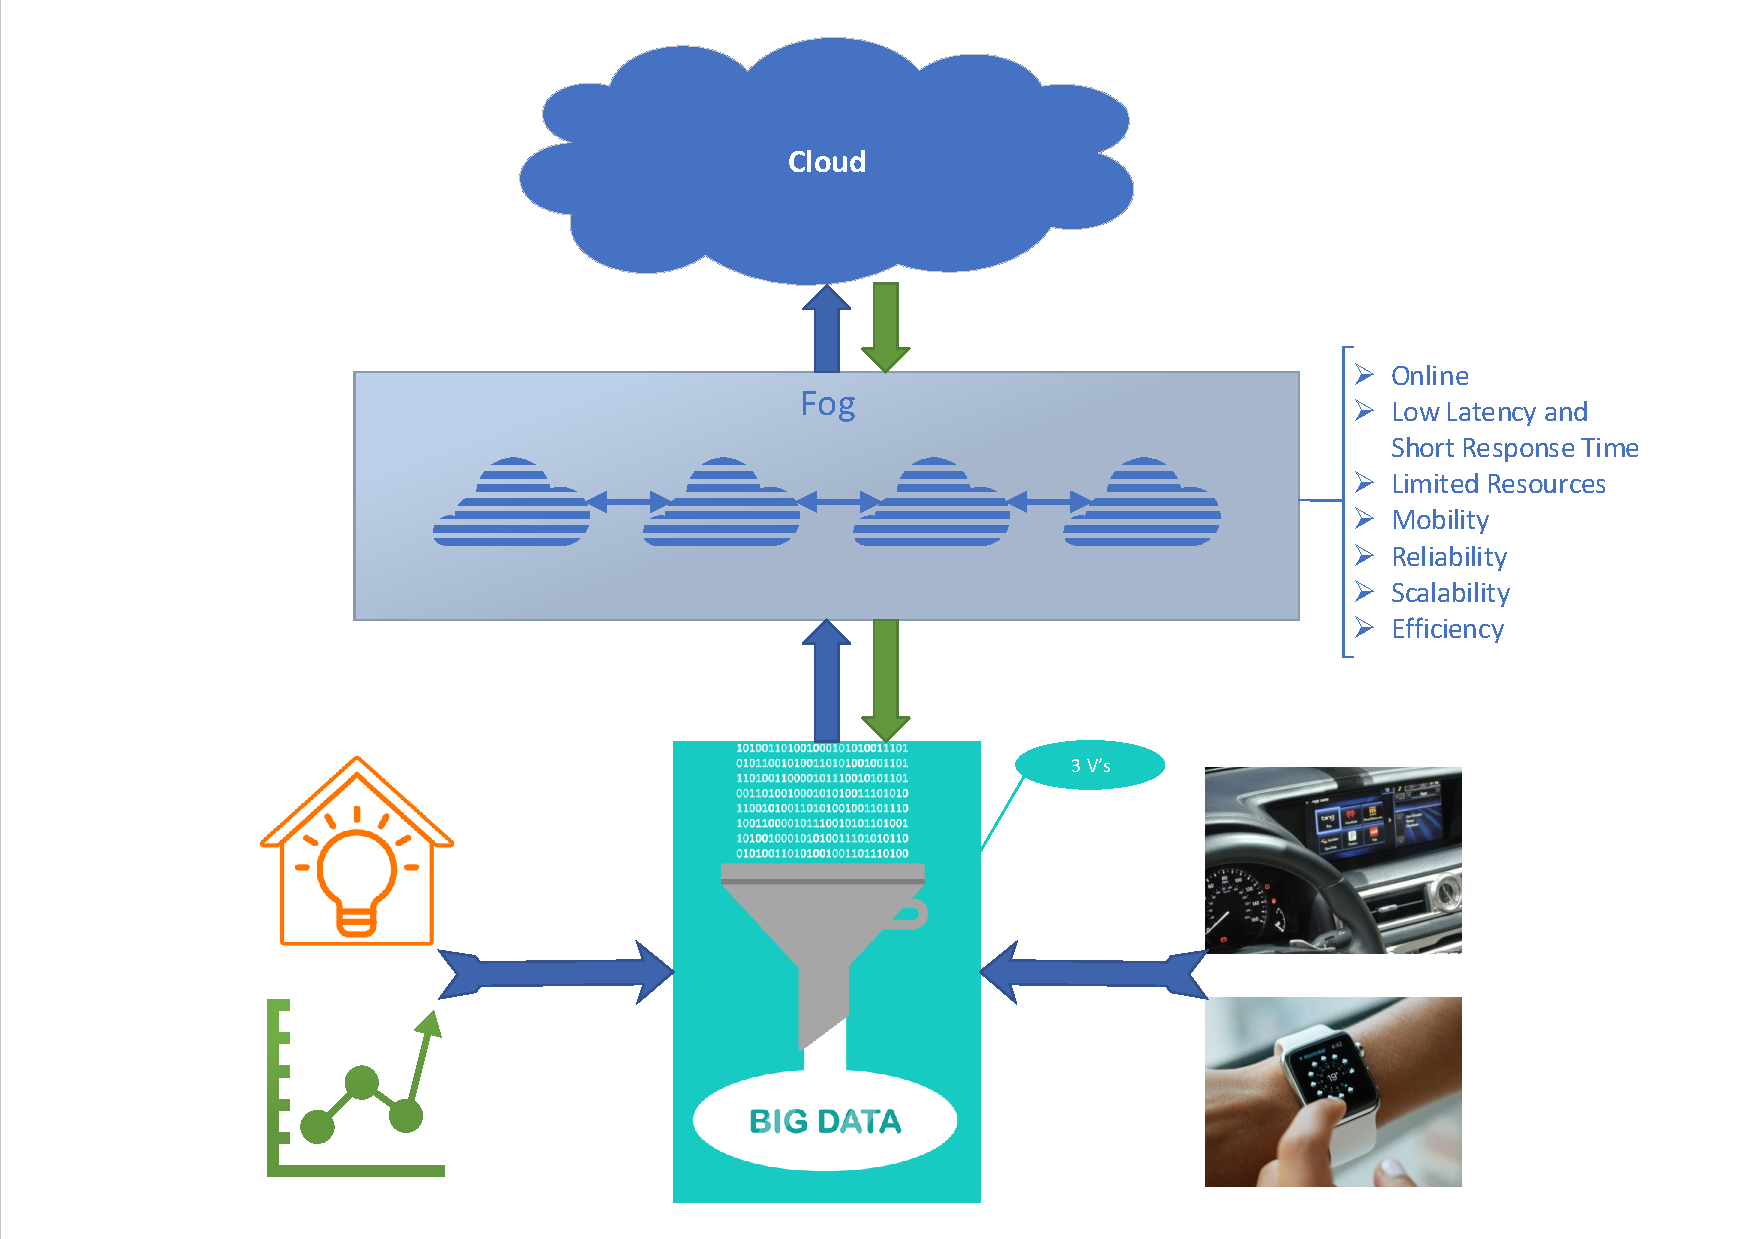
\includegraphics[width = \textwidth]{figs/Data_Stream_Processing_in_Fog_Computing.pdf}
  \end{frame}

  \note{proposed by Cisco in 2012}
  \note{Data locality: move the processes, decrease latency}
  \note{tradeoff between accuracy and response time}

  %%% Problem %%%%%%%%%%%%%%%%%%%%%%%%%%%%%%%%%%%%%%%%%%%%%%%%
  \section[Problem]{Problem}
  \begin{frame}
    \frametitle{Problem Specification}
    Early detection of epilepsy seizures using EEG timeseries data
    %todo cite the waterloo thesis

    \begin{itemize}
      \item Stream processing on the edge
      \item Clustering in the cloud
    \end{itemize}
  \end{frame}

  \begin{frame}
    \frametitle{Dataset}
  % todo cite the two data refs
  \begin{itemize}
    \item \(500\) individuals, each with \(4097\) data points for \(23.5s\) %todo cite the original paper
    \item \(23 \times 500 = 11500\) records, each record contains \(178\) data points (columns) for \(1\) second
    \item Restructured to \texttt{(time, value)} tuples to be used as a stream \(\Rightarrow 11500 \times 178 = 2\,047\,000\) tuples (windows of \(178\))
    \item \(5\) classes \rightarrow \: \(2\) classes (binary)
  \end{itemize}

  \begin{table}
    % \caption{Largest cities in the world (source: Wikipedia)}
    \addfontfeatures{Numbers={Lining,Tabular}}
    {\begin{tabular}{@{} lrrr @{}}
      \toprule
       & Total & Positive & Negative\\
      \midrule
      Training & 7\,000 & 1\,392 & 5\,608\\
      Test & 4\,500& 908 & 3\,592\\
      \addlinespace
      & 11\,500 & 2\,300 & 9\,200\\
      \bottomrule
    \end{tabular}}
  \end{table}

  \end{frame}

  \section{Methodology}
  %%% Edge Computing %%%%%%%%%%%%%%%%%%%%%%%%%%%%%%%%%%%%%%%%%%%%%%%%
  \subsection{Edge Computing}
  \begin{frame}
    \frametitle{Stream Processing at the Edge}
  
    \alert{Goal} Filter the stream for out-of-range tuples/anomalies
    \begin{itemize}
      \item light-weight on resources
      \item fast
    \end{itemize}

    Different statistical measures: variance, skewness, kurtosis

    % \begin{columns}[T,onlytextwidth]
      
    % % \column{0.5\textwidth}
    %   \column{0.5\textwidth}
      
      \metroset{block=fill}
      \begin{exampleblock}{Selected measure}
        \begin{equation*}
          \sqrt{\sum_{i=2}^{n}{(X_i - X_{i-1})^2}}
        \end{equation*}
      \end{exampleblock}
      
    % \end{columns}
    
  \end{frame}

  \note{The first four standardized moments except mean}

  \begin{frame}
    \frametitle{Results}
  
    
  
  \end{frame}


  %%% Clustering in the Cloud %%%%%%%%%%%%%%%%%%%%%%%%%%%%%%%%%%%%%%%%%%%%%%%%
  \subsection{Cloud Computing}
  \begin{frame}
    \frametitle{Clustering in the Cloud}
  
    
  
  \end{frame}


  \begin{frame}
    \frametitle{Results}
  
    
  
  \end{frame}


  %%% Conclusion %%%%%%%%%%%%%%%%%%%%%%%%%%%%%%%%%%%%%%%%%%%%%%%%
  \section{Conclusion}
  \begin{frame}
    \frametitle{Limitations and Future Work}
    \begin{itemize}
      \item Tests with more than one sensor
      \item Introducing a publish-subscribe platform such as Apache Kafka, IBM Watson IoT Hub, etc. (e.g. using MQTT as the protocol)
    \end{itemize}
    
  
  \end{frame}






  %%% Thank you %%%%%%%%%%%%%%%%%%%%%%%%%%%%%%%%%%%%%%%%%%%%%%%%

  \begin{frame}[standout]
    Thank you!
  \end{frame}

  % \begin{frame}
  %   \frametitle{This is the second slide}
  %   \framesubtitle{A bit more information about this}

  %   \begin{itemize}[<+->]
  %     \item The truths of arithmetic which are independent of PA in some 
  %     sense themselves `{contain} essentially {\color{blue}{hidden higher-order}},
  %      or infinitary, concepts'???
  %     \item `Truths in the language of arithmetic which \ldots
  %     \item	That suggests stronger version of Isaacson's thesis. 
  %     \end{itemize}

  %   \begin{equation*}
  %     \symup{e} = \lim_{n\to \infty} \left(1 + \frac{1}{n}\right)^n
  %   \end{equation*}
  %   % \pause
  %   \begin{equation*}
  %     s_{t}=\begin{cases}
  %     \bar{s}, & t\in \left\lbrace 0,\dots, T-1\right\rbrace  \\
  %     \tilde{s}, & t\geq T Q125\% Question \alpha \gamma \varGamma
  %     \end{cases}
  %   \end{equation*} 
  %   %More content goes here
  % \end{frame}
% etc
\end{document}